\documentclass[12pt]{article}

% Ustawienia strony
\usepackage{lipsum}
\usepackage[margin=1.5cm]{geometry}
\usepackage{graphicx}
\usepackage{enumitem}
\usepackage{siunitx}
\usepackage{amsmath}
\usepackage{cancel}
\usepackage{makecell}
\usepackage{mathtools}
\usepackage{floatrow}
\usepackage{caption}
\usepackage[T1]{fontenc}
\usepackage{fancyvrb}
\usepackage[ngerman]{babel} %Deutsche Sprachunterstützung
\usepackage{subcaption}
\usepackage{graphicx}
\fvset{tabsize=4}
\setlist{leftmargin=15pt,labelindent=15pt}
\setlist[enumerate]{noitemsep,wide=0pt, leftmargin=*}
{\setlength{\parindent}{0pt}

% Ustawienia stopki
\usepackage{lastpage}
\usepackage{fancyhdr}
\pagestyle{fancy}
\fancyhf{} % sets both header and footer to nothing
\renewcommand{\headrulewidth}{0pt}
\cfoot{\thepage\ z \pageref{LastPage}}

\begin{document}

\section*{Podstawowe dane}
\begin{figure}[htp]
	\begin{minipage}[t]{0.3\textwidth}
		\textbf{Imie i nazwisko} \\
		\textbf{Data} \\
		\textbf{Tytuł} \\
		\textbf{Numer ćwiczenia}
	\end{minipage}%
	\begin{minipage}[t]{0.6\textwidth}
		Robert Mesek \\
		21.10.2023 \\
		Algorytmy geometryczne \\
		1
	\end{minipage}%
\end{figure}

\section*{Dane techniczne}
\begin{figure}[htp]
	\begin{minipage}[t]{0.3\textwidth}
		\textbf{Procesor} \\
		\textbf{Język} \\
		\textbf{Biblioteki} \\
		\textbf{System operacyjny} \\
		\textbf{Środowisko}

	\end{minipage}%
	\begin{minipage}[t]{0.6\textwidth}
		Intel i7-1165G7 x86\_64 \\
		Python 3.11.5 \\
		NumPy 1.26.0, Pandas 2.1.1, Matplotlib 3.8.0 \\
		WSL Ubuntu 22.04 (MS Windows 10 22H2) \\
		conda 23.5.2
	\end{minipage}%
\end{figure}

\section*{Realizacja ćwiczenia}
\par
Celem ćwiczenia jest sprawdzanie po której stronie prostej znajdują się punkty korzystając z algorytmu wykorzystującego wyznacznik macierzy.

Prostym sposobem do obliczenia, po której stronie prostej znajduje się punkt jest obliczenie iloczynu wektorowego
$\overrightarrow{ab} \times \overrightarrow{ac}$, gdzie $ c = (x,y)$ jest punktem, dla którego poszukujemy wiadomości o lokalizacji względem prostej przechodzącej przez punkty $ a$ i $ b$. Metoda ta jest równoznaczna z obliczeniem wyznacznika macierzy $ 2\times2$:

\begin{gather*}
	\det(a, b, c)= \begin{vmatrix}
		a_{x} - c_{x} & a_{y} - c_{y} \\
		b_{x} - c_{x} & b_{y} - c_{y}
	\end{vmatrix}
	\tag{1}
\end{gather*}


lub wyznacznika macierzy $ 3\times3$:

\begin{gather*}
	\det(a, b, c)= \begin{vmatrix}
		a_{x} & a_{y} & 1 \\
		b_{x} & b_{y} & 1 \\
		c_{x} & c_{y} & 1
	\end{vmatrix}
	\tag{2}
\end{gather*}

Upraszczając tą macierz przez odjęcie drugiego wiersza od trzeciego i odjęcie pierwszego wiersza od drugiego otrzymamy:

\begin{gather*}
	\det(a, b, c)  = \begin{vmatrix}
		a_{x}         & a_{y}         & 1 \\
		b_{x} - a_{x} & b_{y} - a_{y} & 0 \\
		c_{x} - b_{x} & c_{y} - b_{y} & 0
	\end{vmatrix}
	= (b_{x} - a_{x})(c_{y} - b_{y}) - (b_{y} - a_{y})(c_{x} - b_{x})
\end{gather*}

\subsection*{Zbiory punktów}
\par
\verb|points_a| \\
$10^5$ losowych punktów w przestrzeni 2D o współrzędnych z przedziału $x, y \in \left[-1000,1000\right]^{2}$
\begin{figure}[H]
	\centering
	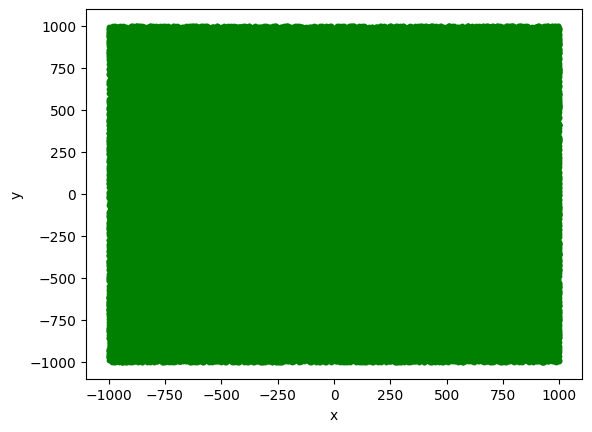
\includegraphics[width=0.7\linewidth]{images/punkty1.png}
\end{figure}

\verb|points_b| \\
$10^5$ losowych punktów w przestrzeni 2D o współrzędnych z przedziału $ x, y \in \left[-10^{14},10^{14}\right]^{2}$
\begin{figure}[H]
	\centering
	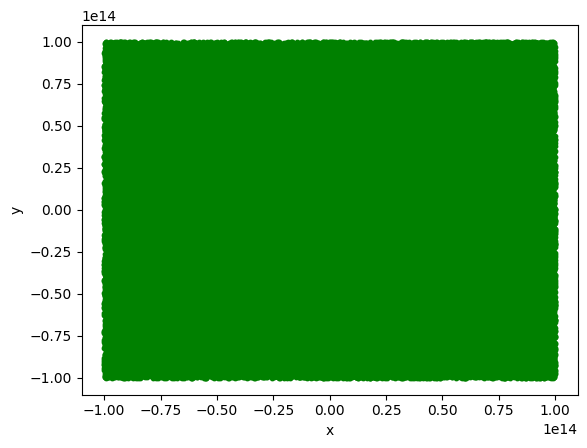
\includegraphics[width=0.7\linewidth]{images/punkty2.png}
\end{figure}

\newpage

\par
\verb|points_c| \\
$1000$ losowych punktów w przestrzeni 2D leżących na okręgu o środku $ O = (0,0)$ i promieniu $ R = 100$
\begin{figure}[H]
	\centering
	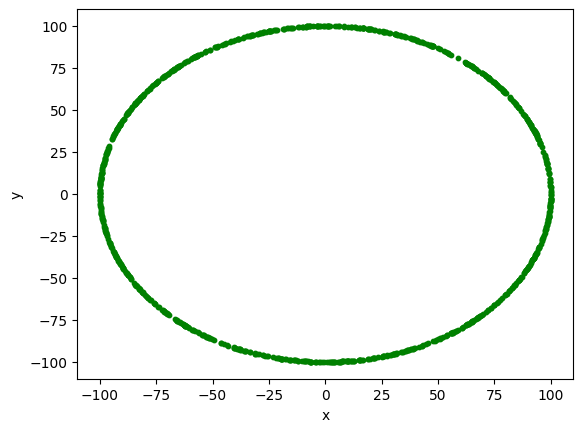
\includegraphics[width=0.7\linewidth]{images/punkty3.png}
\end{figure}

\par
\verb|points_d| \\
$1000$ losowych punktów w przestrzeni 2D o współrzędnej z przedziału $ x \in \langle -1000,1000 \rangle$ leżących na prostej wyznaczonej przez wektor $ \overrightarrow{ab}$. Punkty $ a = (-1.0, 0.0)$ oraz $ b = (1.0, 0.1)$
\begin{figure}[H]
	\centering
	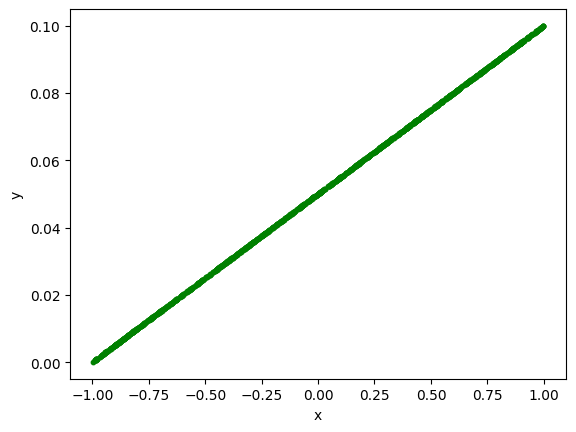
\includegraphics[width=0.7\linewidth]{images/punkty4.png}
\end{figure}

\newpage

\subsection*{Sposoby liczenia wyznacznika}
\paragraph*{Macierz 3x3}
\begin{Verbatim}
def mat_det_3x3(a, b, c):
	"""
	Obliczanie wyznacznika macierzy 3x3 bez użycia funkcji bibliotecznych
	:param a: krotka współrzędnych (x, y) pierwszego punktu tworzącego naszą prostą
	:param b: krotka współrzędnych (x, y) drugiego punktu tworzącego naszą prostą
	:param c: krotka współrzędnych (x, y) punktu, którego położenie względem
	          prostej chcemy znaleźć
	:return: wartość wyznacznika macierzy
	"""
	a_x, a_y = a
	b_x, b_y = b
	c_x, c_y = c
	return (b_x - a_x) * (c_y - b_y) - (b_y - a_y) * (c_x - b_x)
\end{Verbatim}

\paragraph*{Macierz 3x3 biblioteczna}
\begin{Verbatim}
def mat_det_3x3_lib(a, b, c):
	"""
	Obliczanie wyznacznika macierzy 3x3 z użyciem funkcji bibliotecznych
	:param a: krotka współrzędnych (x, y) pierwszego punktu tworzącego naszą prostą
	:param b: krotka współrzędnych (x, y) drugiego punktu tworzącego naszą prostą
	:param c: krotka współrzędnych (x, y) punktu, którego położenie względem prostej 
	          chcemy znaleźć
	:return: wartość wyznacznika macierzy
	"""
	a_x, a_y = a
	b_x, b_y = b
	c_x, c_y = c
	matrix = np.array(
		[
			[a_x, a_y, 1],
			[b_x, b_y, 1],
			[c_x, c_y, 1],
		]
	)
	return np.linalg.det(matrix)
\end{Verbatim}

\newpage

\paragraph*{Macierz 2x2}
\begin{Verbatim}
def mat_det_2x2(a, b, c):
	"""
	Obliczanie wyznacznika macierzy 2x2 bez użycia funkcji bibliotecznych
	:param a: krotka współrzędnych (x, y) pierwszego punktu tworzącego naszą prostą
	:param b: krotka współrzędnych (x, y) drugiego punktu tworzącego naszą prostą
	:param c: krotka współrzędnych (x, y) punktu, którego położenie względem 
	          prostej chcemy znaleźć
	:return: wartość wyznacznika macierzy
	"""
	a_x, a_y = a
	b_x, b_y = b
	c_x, c_y = c
	return (a_x - c_x) * (b_y - c_y) - (a_y - c_y) * (b_x - c_x)
\end{Verbatim}

\paragraph*{Macierz 2x2 biblioteczna}
\begin{Verbatim}
def mat_det_2x2_lib(a, b, c):
	"""
	Obliczanie wyznacznika macierzy 2x2 z użyciem funkcji bibliotecznych
	:param a: krotka współrzędnych (x, y) pierwszego punktu tworzącego naszą prostą
	:param b: krotka współrzędnych (x, y) drugiego punktu tworzącego naszą prostą
	:param c: krotka współrzędnych (x, y) punktu, którego położenie względem prostej 
	          chcemy znaleźć
	:return: wartość wyznacznika macierzy
	"""
	a_x, a_y = a
	b_x, b_y = b
	c_x, c_y = c
	matrix = np.array(
	[
	[a_x - c_x, a_y - c_y],
	[b_x - c_x, b_y - c_y],
	]
	)
	return np.linalg.det(matrix)
\end{Verbatim}

\newpage

\subsection*{Funkcja użyta do kategoryzowania punktów}
\begin{Verbatim}
def categorize_points(points, a, b, mat_det_func, eps):
	"""
	:param points: tablica punktów w postaci krotek współrzednych
	:param a: krotka współrzędnych oznaczająca początek odcinka
	:param b: krotka współrzędnych oznaczająca koniec odcinka
	:param mat_det_func: funkcja która będzie tutaj używana do obliczenia wyznacznika 
	                     macierzy
	:param eps: epsilon - jak blisko wyznacznik macierzy ma być blisko zera, 
	            aby uznać punkt za leżący na prostej
	:return: 3 tablice zawierające kolejno zbiory punktów: leżące na lewo od prostej, 
	         leżące na prostej, leżące na prawo od prostek
	"""
	classified_points_left = []
	classified_points_mid = []
	classified_points_right = []
	for point in points:
		det = mat_det_func(a, b, point)
		if abs(det) < eps:  # det == 0
			classified_points_mid.append(point)
		elif det > 0:
			classified_points_left.append(point)
		else:
			classified_points_right.append(point)
	return classified_points_left, classified_points_mid, classified_points_right
\end{Verbatim}

\subsection*{Epsilon}
\paragraph*{Granica nierówności przy sprawdzaniu czy punkt leży na prostej} \mbox{}\newline
$\varepsilon$: $0$, $10^{-6}$, $10^{-12}$, $10^{-16}$

\subsection*{Precyzje typu zmiennoprzecinkowego}
\verb*|float64| (domyślny), \verb*|float32|

\newpage

\section*{Analiza wyników}
\subsection*{Znaczenie kolorów}
Punkty różnią się kolorami ze względu na klasyfikację: na lewo od prostej - zielone, na prostej - fioletowe, na prawo - pomarańczowe.

\subsection*{Zbiór A}
\begin{figure}[htp]
	\begin{subfigure}[t]{.45\textwidth}
		\centering
		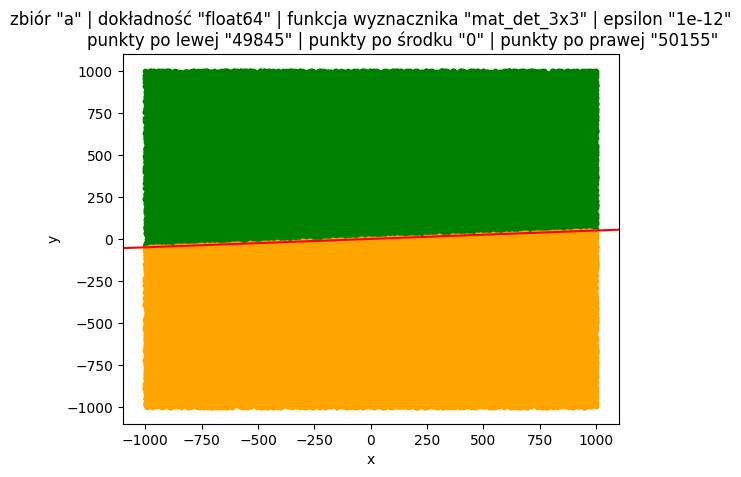
\includegraphics[width=\linewidth]{images/a_f64_3x3_1e-12.png}
		\caption*{Rys. A1}
	\end{subfigure}
	\hfill
	\begin{subfigure}[t]{.45\textwidth}
		\centering
		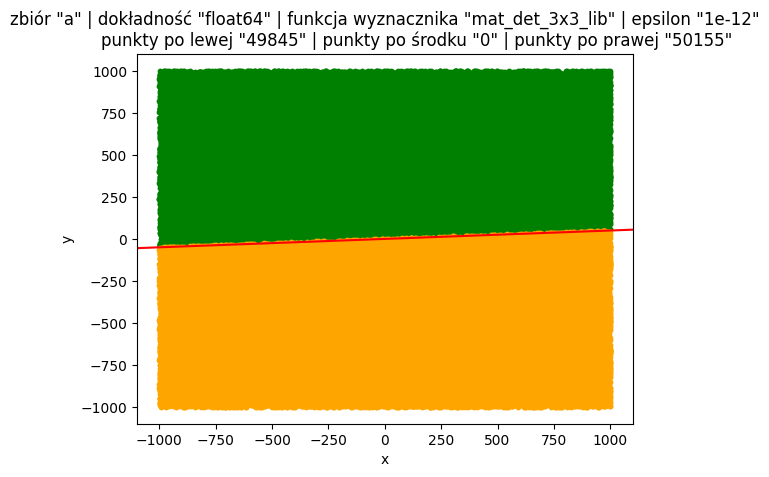
\includegraphics[width=\linewidth]{images/a_f64_3x3-lib_1e-12.png}
		\caption*{Rys. A2}
	\end{subfigure}
	
	\medskip
	
	\begin{subfigure}[t]{.45\textwidth}
		\centering
		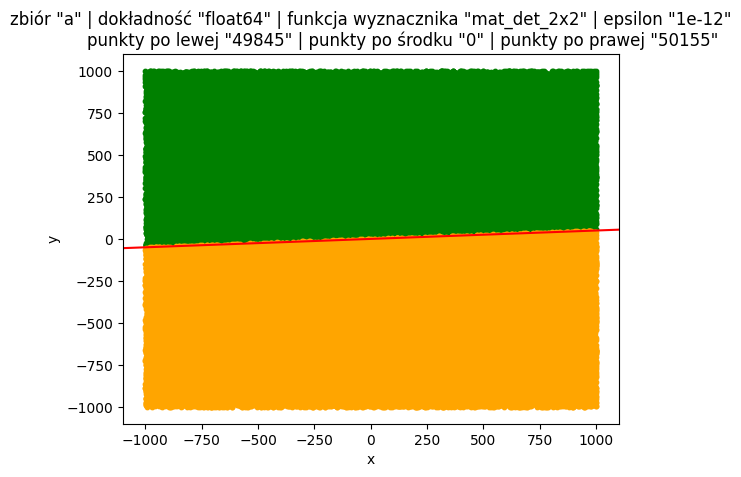
\includegraphics[width=\linewidth]{images/a_f64_2x2_1e-12.png}
		\caption*{Rys. A3}
	\end{subfigure}
	\hfill
	\begin{subfigure}[t]{.45\textwidth}
		\centering
		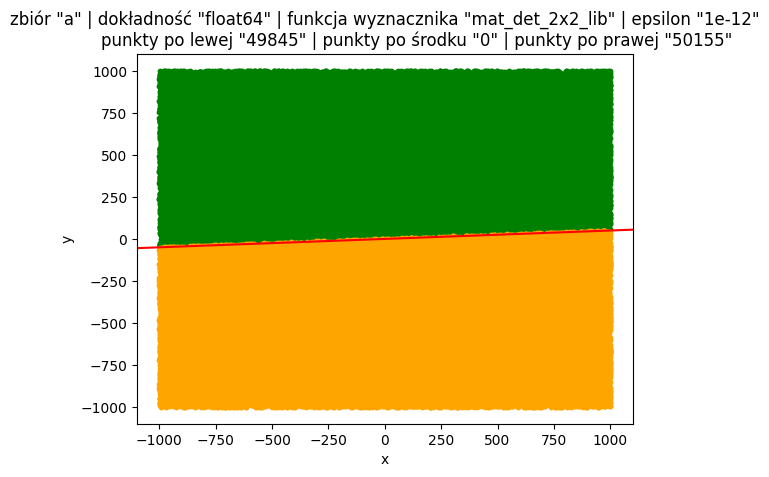
\includegraphics[width=\linewidth]{images/a_f64_2x2-lib_1e-12.png}
		\caption*{Rys. A4}
	\end{subfigure}
\end{figure}
\paragraph{Wyniki A:}
Analizując dane z \textbf{tabeli A} widzimy, że zmiana parametrów oraz algorytmów liczenia wyznacznika nie wpływa na wyniki. Widzimy to na rysunkach \textbf{A1, A2, A3, A4}.

\par
\begin{table}[H]
	\centering
	\begin{tabular}{|c|c|c|c|c|c|c|}
		\hline
		\textbf{\makecell{Zbiór}} & \textbf{\makecell{Dokładność\\float}} & \textbf{\makecell{Wyznacznik}} & \textbf{\makecell{Epsilon}} & \textbf{\makecell{Punktów\\z lewej}} & \textbf{\makecell{Punktów\\po środku}} & \textbf{\makecell{Punktów\\z prawej}} \\ \hline
		a & float64 & mat\_det\_3x3 & 0e+00 & 49915 & 0 & 50085 \\ 
		a & float64 & mat\_det\_3x3 & 1e-06 & 49915 & 0 & 50085 \\ 
		a & float64 & mat\_det\_3x3 & 1e-12 & 49915 & 0 & 50085 \\ 
		a & float64 & mat\_det\_3x3 & 1e-16 & 49915 & 0 & 50085 \\ 
		a & float64 & mat\_det\_3x3\_lib & 0e+00 & 49915 & 0 & 50085 \\ 
		a & float64 & mat\_det\_3x3\_lib & 1e-06 & 49915 & 0 & 50085 \\ 
		a & float64 & mat\_det\_3x3\_lib & 1e-12 & 49915 & 0 & 50085 \\ 
		a & float64 & mat\_det\_3x3\_lib & 1e-16 & 49915 & 0 & 50085 \\ 
		a & float64 & mat\_det\_2x2 & 0e+00 & 49915 & 0 & 50085 \\ 
		a & float64 & mat\_det\_2x2 & 1e-06 & 49915 & 0 & 50085 \\ 
		a & float64 & mat\_det\_2x2 & 1e-12 & 49915 & 0 & 50085 \\ 
		a & float64 & mat\_det\_2x2 & 1e-16 & 49915 & 0 & 50085 \\ 
		a & float64 & mat\_det\_2x2\_lib & 0e+00 & 49915 & 0 & 50085 \\ 
		a & float64 & mat\_det\_2x2\_lib & 1e-06 & 49915 & 0 & 50085 \\ 
		a & float64 & mat\_det\_2x2\_lib & 1e-12 & 49915 & 0 & 50085 \\ 
		a & float64 & mat\_det\_2x2\_lib & 1e-16 & 49915 & 0 & 50085 \\ 
		a & float32 & mat\_det\_3x3 & 0e+00 & 49915 & 0 & 50085 \\ 
		a & float32 & mat\_det\_3x3 & 1e-06 & 49915 & 0 & 50085 \\ 
		a & float32 & mat\_det\_3x3 & 1e-12 & 49915 & 0 & 50085 \\ 
		a & float32 & mat\_det\_3x3 & 1e-16 & 49915 & 0 & 50085 \\ 
		a & float32 & mat\_det\_3x3\_lib & 0e+00 & 49915 & 0 & 50085 \\ 
		a & float32 & mat\_det\_3x3\_lib & 1e-06 & 49915 & 0 & 50085 \\ 
		a & float32 & mat\_det\_3x3\_lib & 1e-12 & 49915 & 0 & 50085 \\ 
		a & float32 & mat\_det\_3x3\_lib & 1e-16 & 49915 & 0 & 50085 \\ 
		a & float32 & mat\_det\_2x2 & 0e+00 & 49915 & 0 & 50085 \\ 
		a & float32 & mat\_det\_2x2 & 1e-06 & 49915 & 0 & 50085 \\ 
		a & float32 & mat\_det\_2x2 & 1e-12 & 49915 & 0 & 50085 \\ 
		a & float32 & mat\_det\_2x2 & 1e-16 & 49915 & 0 & 50085 \\ 
		a & float32 & mat\_det\_2x2\_lib & 0e+00 & 49915 & 0 & 50085 \\ 
		a & float32 & mat\_det\_2x2\_lib & 1e-06 & 49915 & 0 & 50085 \\ 
		a & float32 & mat\_det\_2x2\_lib & 1e-12 & 49915 & 0 & 50085 \\ 
		a & float32 & mat\_det\_2x2\_lib & 1e-16 & 49915 & 0 & 50085 \\ \hline
	\end{tabular}
	\caption*{Tabela A}
\end{table}

\newpage

\subsection*{Zbiór B}
\begin{figure}[htp]
	\begin{subfigure}[t]{.45\textwidth}
		\centering
		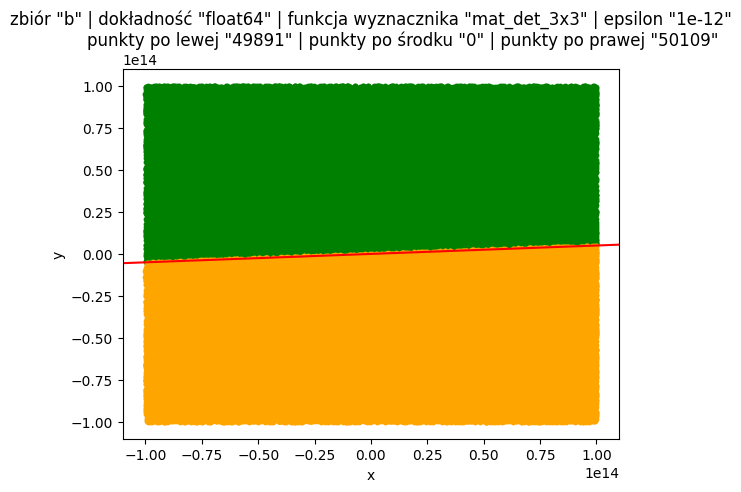
\includegraphics[width=\linewidth]{images/b_f64_3x3_1e-12.png}
		\caption*{Rys. B1}
	\end{subfigure}
	\hfill
	\begin{subfigure}[t]{.45\textwidth}
		\centering
		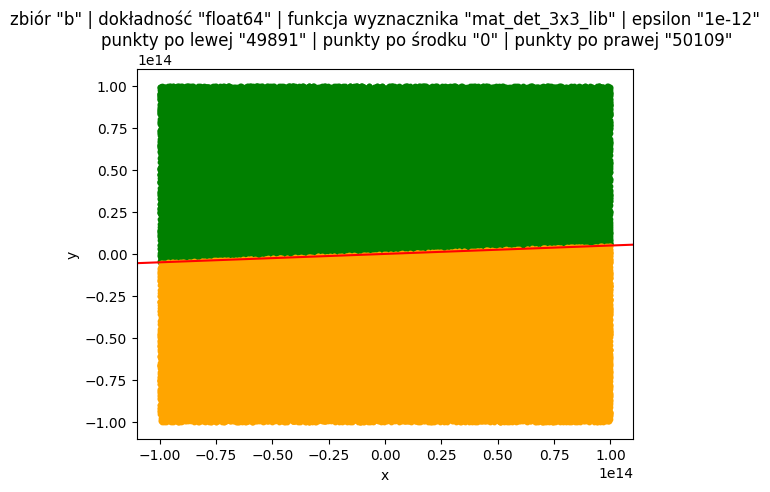
\includegraphics[width=\linewidth]{images/b_f64_3x3-lib_1e-12.png}
		\caption*{Rys. B2}
	\end{subfigure}
	
	\medskip
	
	\begin{subfigure}[t]{.45\textwidth}
		\centering
		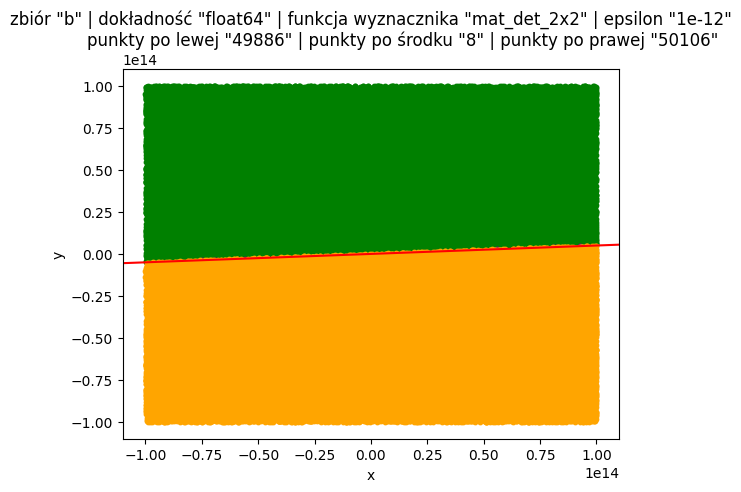
\includegraphics[width=\linewidth]{images/b_f64_2x2_1e-12.png}
		\caption*{Rys. B3}
	\end{subfigure}
	\hfill
	\begin{subfigure}[t]{.45\textwidth}
		\centering
		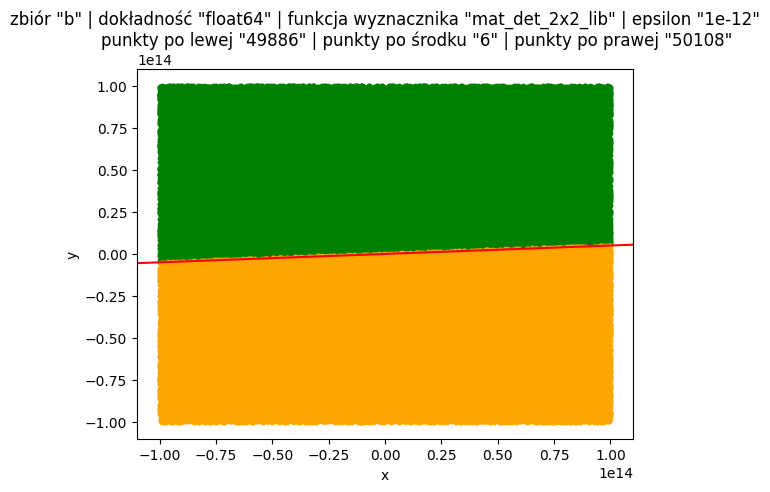
\includegraphics[width=\linewidth]{images/b_f64_2x2-lib_1e-12.png}
		\caption*{Rys. B4}
	\end{subfigure}
\end{figure}
\paragraph{Wyniki B:}
Analizując dane z \textbf{tabeli B} widzimy, że zmiana parametrów oraz algorytmów liczenia wyznacznika minimalnie wpływa na wyniki: $\approx 10$ różnic dla $50000$.

\par
\begin{table}[H]
	\centering
	\begin{tabular}{|c|c|c|c|c|c|c|}
		\hline
		\textbf{\makecell{Zbiór}} & \textbf{\makecell{Dokładność\\float}} & \textbf{\makecell{Wyznacznik}} & \textbf{\makecell{Epsilon}} & \textbf{\makecell{Punktów\\z lewej}} & \textbf{\makecell{Punktów\\po środku}} & \textbf{\makecell{Punktów\\z prawej}} \\ \hline
		b & float64 & mat\_det\_3x3 & 0e+00 & 49739 & 0 & 50261 \\ 
		b & float64 & mat\_det\_3x3 & 1e-06 & 49739 & 0 & 50261 \\ 
		b & float64 & mat\_det\_3x3 & 1e-12 & 49739 & 0 & 50261 \\ 
		b & float64 & mat\_det\_3x3 & 1e-16 & 49739 & 0 & 50261 \\ 
		b & float64 & mat\_det\_3x3\_lib & 0e+00 & 49739 & 0 & 50261 \\ 
		b & float64 & mat\_det\_3x3\_lib & 1e-06 & 49739 & 0 & 50261 \\ 
		b & float64 & mat\_det\_3x3\_lib & 1e-12 & 49739 & 0 & 50261 \\ 
		b & float64 & mat\_det\_3x3\_lib & 1e-16 & 49739 & 0 & 50261 \\ 
		b & float64 & mat\_det\_2x2 & 0e+00 & 49735 & 0 & 50265 \\ 
		b & float64 & mat\_det\_2x2 & 1e-06 & 49735 & 7 & 50258 \\ 
		b & float64 & mat\_det\_2x2 & 1e-12 & 49735 & 7 & 50258 \\ 
		b & float64 & mat\_det\_2x2 & 1e-16 & 49735 & 7 & 50258 \\ 
		b & float64 & mat\_det\_2x2\_lib & 0e+00 & 49735 & 0 & 50265 \\ 
		b & float64 & mat\_det\_2x2\_lib & 1e-06 & 49735 & 5 & 50260 \\ 
		b & float64 & mat\_det\_2x2\_lib & 1e-12 & 49735 & 5 & 50260 \\ 
		b & float64 & mat\_det\_2x2\_lib & 1e-16 & 49735 & 5 & 50260 \\ 
		b & float32 & mat\_det\_3x3 & 0e+00 & 49739 & 0 & 50261 \\ 
		b & float32 & mat\_det\_3x3 & 1e-06 & 49739 & 0 & 50261 \\ 
		b & float32 & mat\_det\_3x3 & 1e-12 & 49739 & 0 & 50261 \\ 
		b & float32 & mat\_det\_3x3 & 1e-16 & 49739 & 0 & 50261 \\ 
		b & float32 & mat\_det\_3x3\_lib & 0e+00 & 49739 & 0 & 50261 \\ 
		b & float32 & mat\_det\_3x3\_lib & 1e-06 & 49739 & 0 & 50261 \\ 
		b & float32 & mat\_det\_3x3\_lib & 1e-12 & 49739 & 0 & 50261 \\ 
		b & float32 & mat\_det\_3x3\_lib & 1e-16 & 49739 & 0 & 50261 \\ 
		b & float32 & mat\_det\_2x2 & 0e+00 & 49733 & 0 & 50267 \\ 
		b & float32 & mat\_det\_2x2 & 1e-06 & 49733 & 9 & 50258 \\ 
		b & float32 & mat\_det\_2x2 & 1e-12 & 49733 & 9 & 50258 \\ 
		b & float32 & mat\_det\_2x2 & 1e-16 & 49733 & 9 & 50258 \\ 
		b & float32 & mat\_det\_2x2\_lib & 0e+00 & 49736 & 0 & 50264 \\ 
		b & float32 & mat\_det\_2x2\_lib & 1e-06 & 49736 & 6 & 50258 \\ 
		b & float32 & mat\_det\_2x2\_lib & 1e-12 & 49736 & 6 & 50258 \\ 
		b & float32 & mat\_det\_2x2\_lib & 1e-16 & 49736 & 6 & 50258 \\ \hline
	\end{tabular}
	\caption*{Tabela B}
\end{table}

\newpage

\subsection*{Zbiór C}
\begin{figure}[htp]
	\begin{subfigure}[t]{.45\textwidth}
		\centering
		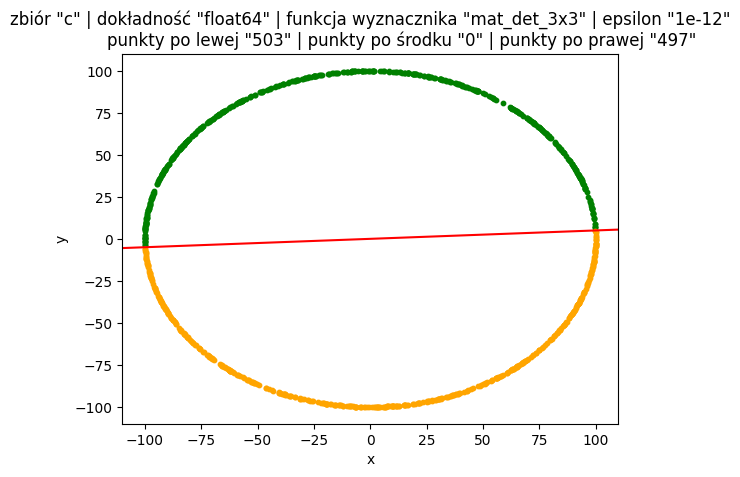
\includegraphics[width=\linewidth]{images/c_f64_3x3_1e-12.png}
		\caption*{Rys. C1}
	\end{subfigure}
	\hfill
	\begin{subfigure}[t]{.45\textwidth}
		\centering
		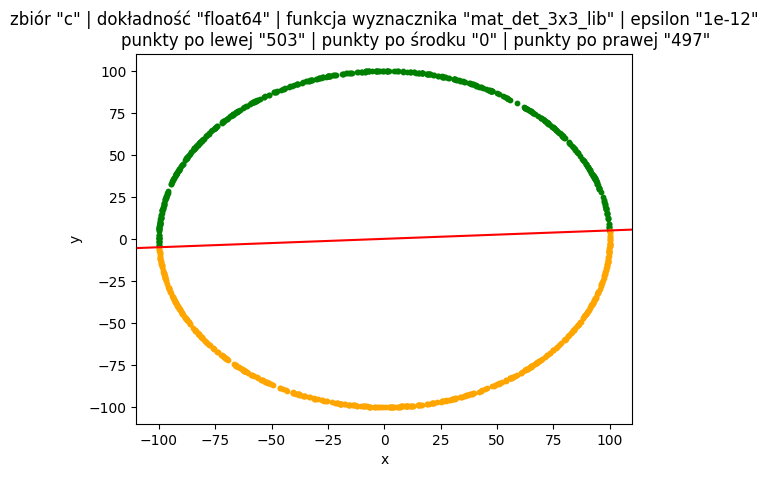
\includegraphics[width=\linewidth]{images/c_f64_3x3-lib_1e-12.png}
		\caption*{Rys. C2}
	\end{subfigure}
	
	\medskip
	
	\begin{subfigure}[t]{.45\textwidth}
		\centering
		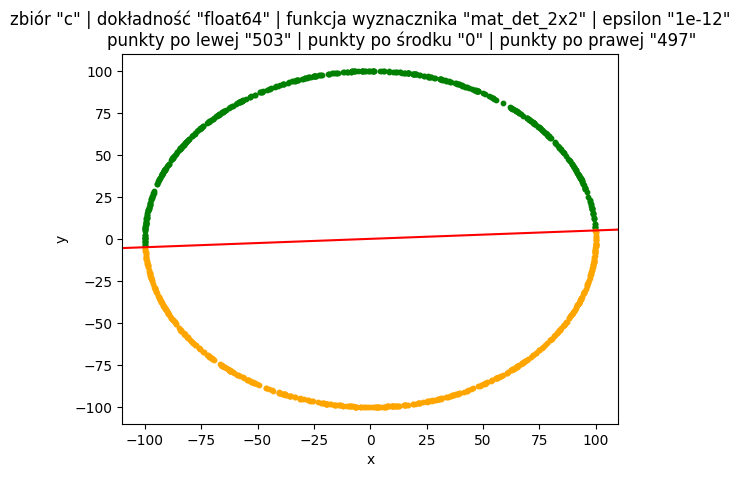
\includegraphics[width=\linewidth]{images/c_f64_2x2_1e-12.png}
		\caption*{Rys. C3}
	\end{subfigure}
	\hfill
	\begin{subfigure}[t]{.45\textwidth}
		\centering
		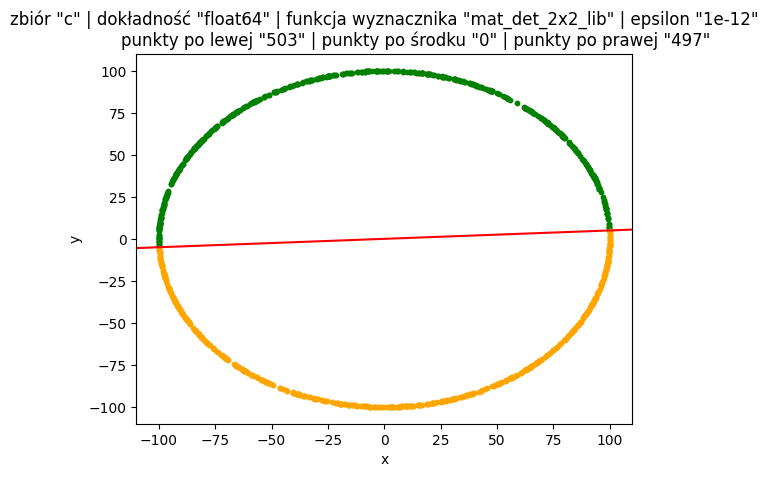
\includegraphics[width=\linewidth]{images/c_f64_2x2-lib_1e-12.png}
		\caption*{Rys. C4}
	\end{subfigure}
\end{figure}
\paragraph{Wyniki C:}
Analizując dane z \textbf{tabeli C} widzimy, że zmiana parametrów oraz algorytmów liczenia wyznacznika nie wpływa na wyniki. Widzimy to na rysunkach \textbf{C1, C2, C3, C4}.

\par
\begin{table}[H]
	\centering
	\begin{tabular}{|c|c|c|c|c|c|c|}
		\hline
		\textbf{\makecell{Zbiór}} & \textbf{\makecell{Dokładność\\float}} & \textbf{\makecell{Wyznacznik}} & \textbf{\makecell{Epsilon}} & \textbf{\makecell{Punktów\\z lewej}} & \textbf{\makecell{Punktów\\po środku}} & \textbf{\makecell{Punktów\\z prawej}} \\ \hline
		c & float64 & mat\_det\_3x3 & 0e+00 & 503 & 0 & 497 \\ 
		c & float64 & mat\_det\_3x3 & 1e-06 & 503 & 0 & 497 \\ 
		c & float64 & mat\_det\_3x3 & 1e-12 & 503 & 0 & 497 \\ 
		c & float64 & mat\_det\_3x3 & 1e-16 & 503 & 0 & 497 \\ 
		c & float64 & mat\_det\_3x3\_lib & 0e+00 & 503 & 0 & 497 \\ 
		c & float64 & mat\_det\_3x3\_lib & 1e-06 & 503 & 0 & 497 \\ 
		c & float64 & mat\_det\_3x3\_lib & 1e-12 & 503 & 0 & 497 \\ 
		c & float64 & mat\_det\_3x3\_lib & 1e-16 & 503 & 0 & 497 \\ 
		c & float64 & mat\_det\_2x2 & 0e+00 & 503 & 0 & 497 \\ 
		c & float64 & mat\_det\_2x2 & 1e-06 & 503 & 0 & 497 \\ 
		c & float64 & mat\_det\_2x2 & 1e-12 & 503 & 0 & 497 \\ 
		c & float64 & mat\_det\_2x2 & 1e-16 & 503 & 0 & 497 \\ 
		c & float64 & mat\_det\_2x2\_lib & 0e+00 & 503 & 0 & 497 \\ 
		c & float64 & mat\_det\_2x2\_lib & 1e-06 & 503 & 0 & 497 \\ 
		c & float64 & mat\_det\_2x2\_lib & 1e-12 & 503 & 0 & 497 \\ 
		c & float64 & mat\_det\_2x2\_lib & 1e-16 & 503 & 0 & 497 \\ 
		c & float32 & mat\_det\_3x3 & 0e+00 & 503 & 0 & 497 \\ 
		c & float32 & mat\_det\_3x3 & 1e-06 & 503 & 0 & 497 \\ 
		c & float32 & mat\_det\_3x3 & 1e-12 & 503 & 0 & 497 \\ 
		c & float32 & mat\_det\_3x3 & 1e-16 & 503 & 0 & 497 \\ 
		c & float32 & mat\_det\_3x3\_lib & 0e+00 & 503 & 0 & 497 \\ 
		c & float32 & mat\_det\_3x3\_lib & 1e-06 & 503 & 0 & 497 \\ 
		c & float32 & mat\_det\_3x3\_lib & 1e-12 & 503 & 0 & 497 \\ 
		c & float32 & mat\_det\_3x3\_lib & 1e-16 & 503 & 0 & 497 \\ 
		c & float32 & mat\_det\_2x2 & 0e+00 & 503 & 0 & 497 \\ 
		c & float32 & mat\_det\_2x2 & 1e-06 & 503 & 0 & 497 \\ 
		c & float32 & mat\_det\_2x2 & 1e-12 & 503 & 0 & 497 \\ 
		c & float32 & mat\_det\_2x2 & 1e-16 & 503 & 0 & 497 \\ 
		c & float32 & mat\_det\_2x2\_lib & 0e+00 & 503 & 0 & 497 \\ 
		c & float32 & mat\_det\_2x2\_lib & 1e-06 & 503 & 0 & 497 \\ 
		c & float32 & mat\_det\_2x2\_lib & 1e-12 & 503 & 0 & 497 \\ 
		c & float32 & mat\_det\_2x2\_lib & 1e-16 & 503 & 0 & 497 \\ \hline
	\end{tabular}
	\caption*{Tabela C}
\end{table}

\newpage

\subsection*{Zbiór D}
\begin{figure}[htp]
	\begin{subfigure}[t]{.45\textwidth}
		\centering
		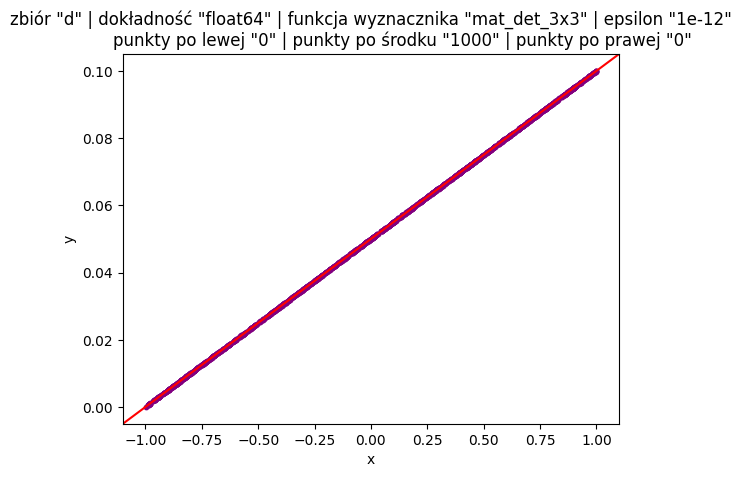
\includegraphics[width=\linewidth]{images/d_f64_3x3_1e-12.png}
		\caption*{Rys. D1}
	\end{subfigure}
	\hfill
	\begin{subfigure}[t]{.45\textwidth}
		\centering
		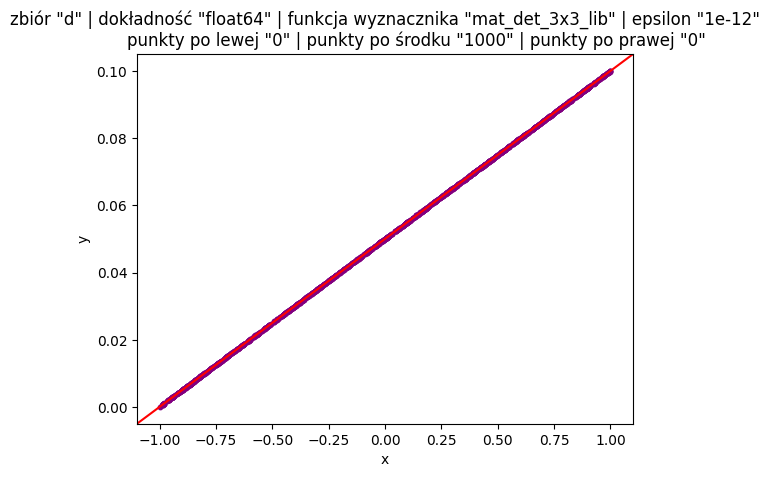
\includegraphics[width=\linewidth]{images/d_f64_3x3-lib_1e-12.png}
		\caption*{Rys. D2}
	\end{subfigure}
	
	\medskip
	
	\begin{subfigure}[t]{.45\textwidth}
		\centering
		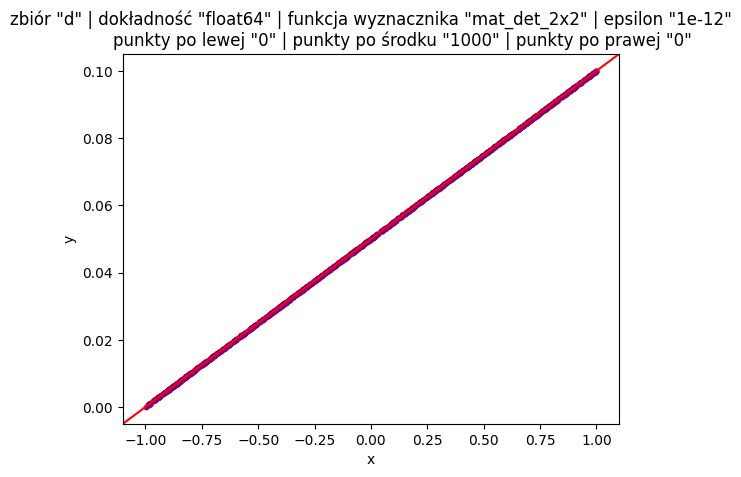
\includegraphics[width=\linewidth]{images/d_f64_2x2_1e-12.png}
		\caption*{Rys. D3}
	\end{subfigure}
	\hfill
	\begin{subfigure}[t]{.45\textwidth}
		\centering
		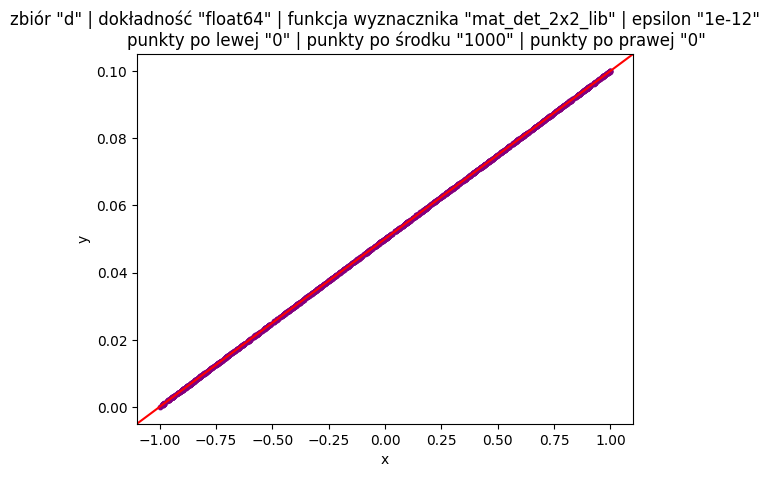
\includegraphics[width=\linewidth]{images/d_f64_2x2-lib_1e-12.png}
		\caption*{Rys. D4}
	\end{subfigure}
\end{figure}

\paragraph{Wyniki D:}
Analizując dane z \textbf{tabeli D} widzimy, dwa czynniki zmieniające nasze wyniki. \\
1) Dla $\varepsilon = 0$ w zależności od innych parametrów nasze wyniki zmieniają się. Jest to jednak oczekiwane zachowanie, ponieważ porównujemy liczby zmiennoprzecinkowe wprost do zera, na co trzeba uważać podczas implementacji algorytmów.

\mbox{}\newline
2) Dla dokładności typu zmiennoprzecinkowego ustawionego na \verb*|float32| stosowanie bardzo małego $\varepsilon$ ($10^{-12},\ 10^{-16}$) widzimy w \textbf{tabeli D}, że wyniki różnią się dla odpowiednich parametrów dla dokładności \verb*|float64|. 

\par
\begin{table}[H]
	\centering
	\begin{tabular}{|c|c|c|c|c|c|c|}
		\hline
		\textbf{\makecell{Zbiór}} & \textbf{\makecell{Dokładność\\float}} & \textbf{\makecell{Wyznacznik}} & \textbf{\makecell{Epsilon}} & \textbf{\makecell{Punktów\\z lewej}} & \textbf{\makecell{Punktów\\po środku}} & \textbf{\makecell{Punktów\\z prawej}} \\ \hline
		d & float64 & mat\_det\_3x3 & 0e+00 & 163 & 0 & 837 \\ 
		d & float64 & mat\_det\_3x3 & 1e-06 & 0 & 1000 & 0 \\ 
		d & float64 & mat\_det\_3x3 & 1e-12 & 0 & 1000 & 0 \\ 
		d & float64 & mat\_det\_3x3 & 1e-16 & 0 & 1000 & 0 \\ 
		d & float64 & mat\_det\_3x3\_lib & 0e+00 & 197 & 0 & 803 \\ 
		d & float64 & mat\_det\_3x3\_lib & 1e-06 & 0 & 1000 & 0 \\ 
		d & float64 & mat\_det\_3x3\_lib & 1e-12 & 0 & 1000 & 0 \\ 
		d & float64 & mat\_det\_3x3\_lib & 1e-16 & 0 & 1000 & 0 \\ 
		d & float64 & mat\_det\_2x2 & 0e+00 & 345 & 0 & 655 \\ 
		d & float64 & mat\_det\_2x2 & 1e-06 & 0 & 1000 & 0 \\ 
		d & float64 & mat\_det\_2x2 & 1e-12 & 0 & 1000 & 0 \\ 
		d & float64 & mat\_det\_2x2 & 1e-16 & 0 & 1000 & 0 \\ 
		d & float64 & mat\_det\_2x2\_lib & 0e+00 & 338 & 0 & 662 \\ 
		d & float64 & mat\_det\_2x2\_lib & 1e-06 & 0 & 1000 & 0 \\ 
		d & float64 & mat\_det\_2x2\_lib & 1e-12 & 0 & 1000 & 0 \\ 
		d & float64 & mat\_det\_2x2\_lib & 1e-16 & 0 & 1000 & 0 \\ 
		d & float32 & mat\_det\_3x3 & 0e+00 & 440 & 0 & 560 \\ 
		d & float32 & mat\_det\_3x3 & 1e-06 & 0 & 1000 & 0 \\ 
		d & float32 & mat\_det\_3x3 & 1e-12 & 440 & 154 & 406 \\ 
		d & float32 & mat\_det\_3x3 & 1e-16 & 440 & 154 & 406 \\ 
		d & float32 & mat\_det\_3x3\_lib & 0e+00 & 440 & 0 & 560 \\ 
		d & float32 & mat\_det\_3x3\_lib & 1e-06 & 0 & 1000 & 0 \\ 
		d & float32 & mat\_det\_3x3\_lib & 1e-12 & 440 & 154 & 406 \\ 
		d & float32 & mat\_det\_3x3\_lib & 1e-16 & 440 & 154 & 406 \\ 
		d & float32 & mat\_det\_2x2 & 0e+00 & 440 & 0 & 560 \\ 
		d & float32 & mat\_det\_2x2 & 1e-06 & 0 & 1000 & 0 \\ 
		d & float32 & mat\_det\_2x2 & 1e-12 & 440 & 154 & 406 \\ 
		d & float32 & mat\_det\_2x2 & 1e-16 & 440 & 154 & 406 \\ 
		d & float32 & mat\_det\_2x2\_lib & 0e+00 & 441 & 0 & 559 \\ 
		d & float32 & mat\_det\_2x2\_lib & 1e-06 & 0 & 1000 & 0 \\ 
		d & float32 & mat\_det\_2x2\_lib & 1e-12 & 440 & 154 & 406 \\ 
		d & float32 & mat\_det\_2x2\_lib & 1e-16 & 440 & 154 & 406 \\ \hline
	\end{tabular}
	\caption*{Tabela D}
\end{table}

\newpage

\paragraph{Różnice wykresów dla D}\mbox{}
\begin{figure}[htp]
	\begin{subfigure}[t]{.45\textwidth}
		\centering
		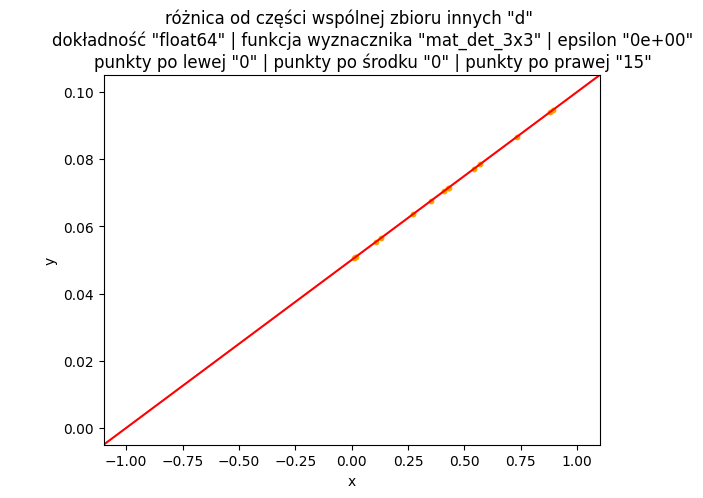
\includegraphics[width=\linewidth]{images/d_diff_1.png}
		\caption*{Rys. D'1}
	\end{subfigure}
	\hfill
	\begin{subfigure}[t]{.45\textwidth}
		\centering
		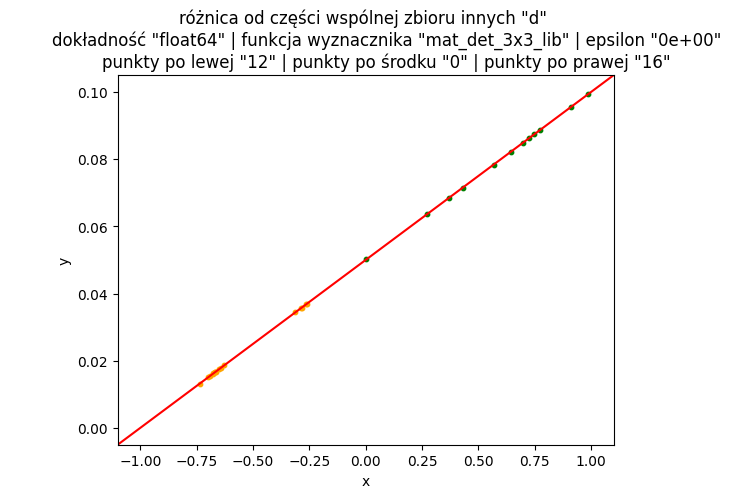
\includegraphics[width=\linewidth]{images/d_diff_2.png}
		\caption*{Rys. D'2}
	\end{subfigure}
	
	\medskip
	
	\begin{subfigure}[t]{.45\textwidth}
		\centering
		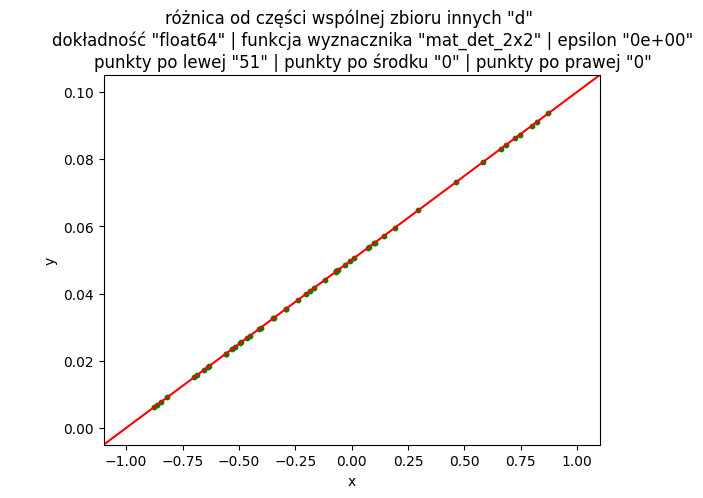
\includegraphics[width=\linewidth]{images/d_diff_3.png}
		\caption*{Rys. D'3}
	\end{subfigure}
	\hfill
	\begin{subfigure}[t]{.45\textwidth}
		\centering
		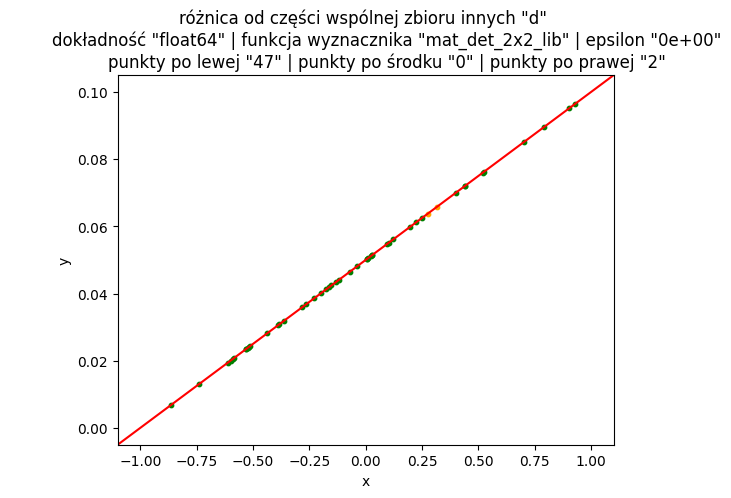
\includegraphics[width=\linewidth]{images/d_diff_4.png}
		\caption*{Rys. D'4}
	\end{subfigure}
\end{figure}

\section*{Wnioski}
\par
Dla zbiorów A, B, C różnice wynikające ze sprawdzanych parametrów są znikome.

\mbox{}\newline
Dla zbioru D możemy zaobserwować, że porównywanie liczb zmiennoprzecinkowych z zerem bez użycia marginesu błędu nie będzie dawało oczekiwanych wyników, ale ciekawszą obserwacją jest fakt, że zmiana dokładności liczb zmiennoprzecinkowych między \verb*|float64|, \verb*|float32| daje obserwowalne pogorszenie dokładności wyników.

Może to być spowodowane faktem, że stosując \verb*|float32| nie możemy dobrze zaprezentować punktów leżących wzdłuż linii. Dlatego musimy zwiększyć $\varepsilon$, aby dostawać oczekiwane wyniki (\textbf{Tabela D}).

\end{document}
